\section{Материалы предварительного проектирования системы}
\subsection{Функциональная схема обработки данных}

\begin{figure}[!htb]
    \centering
    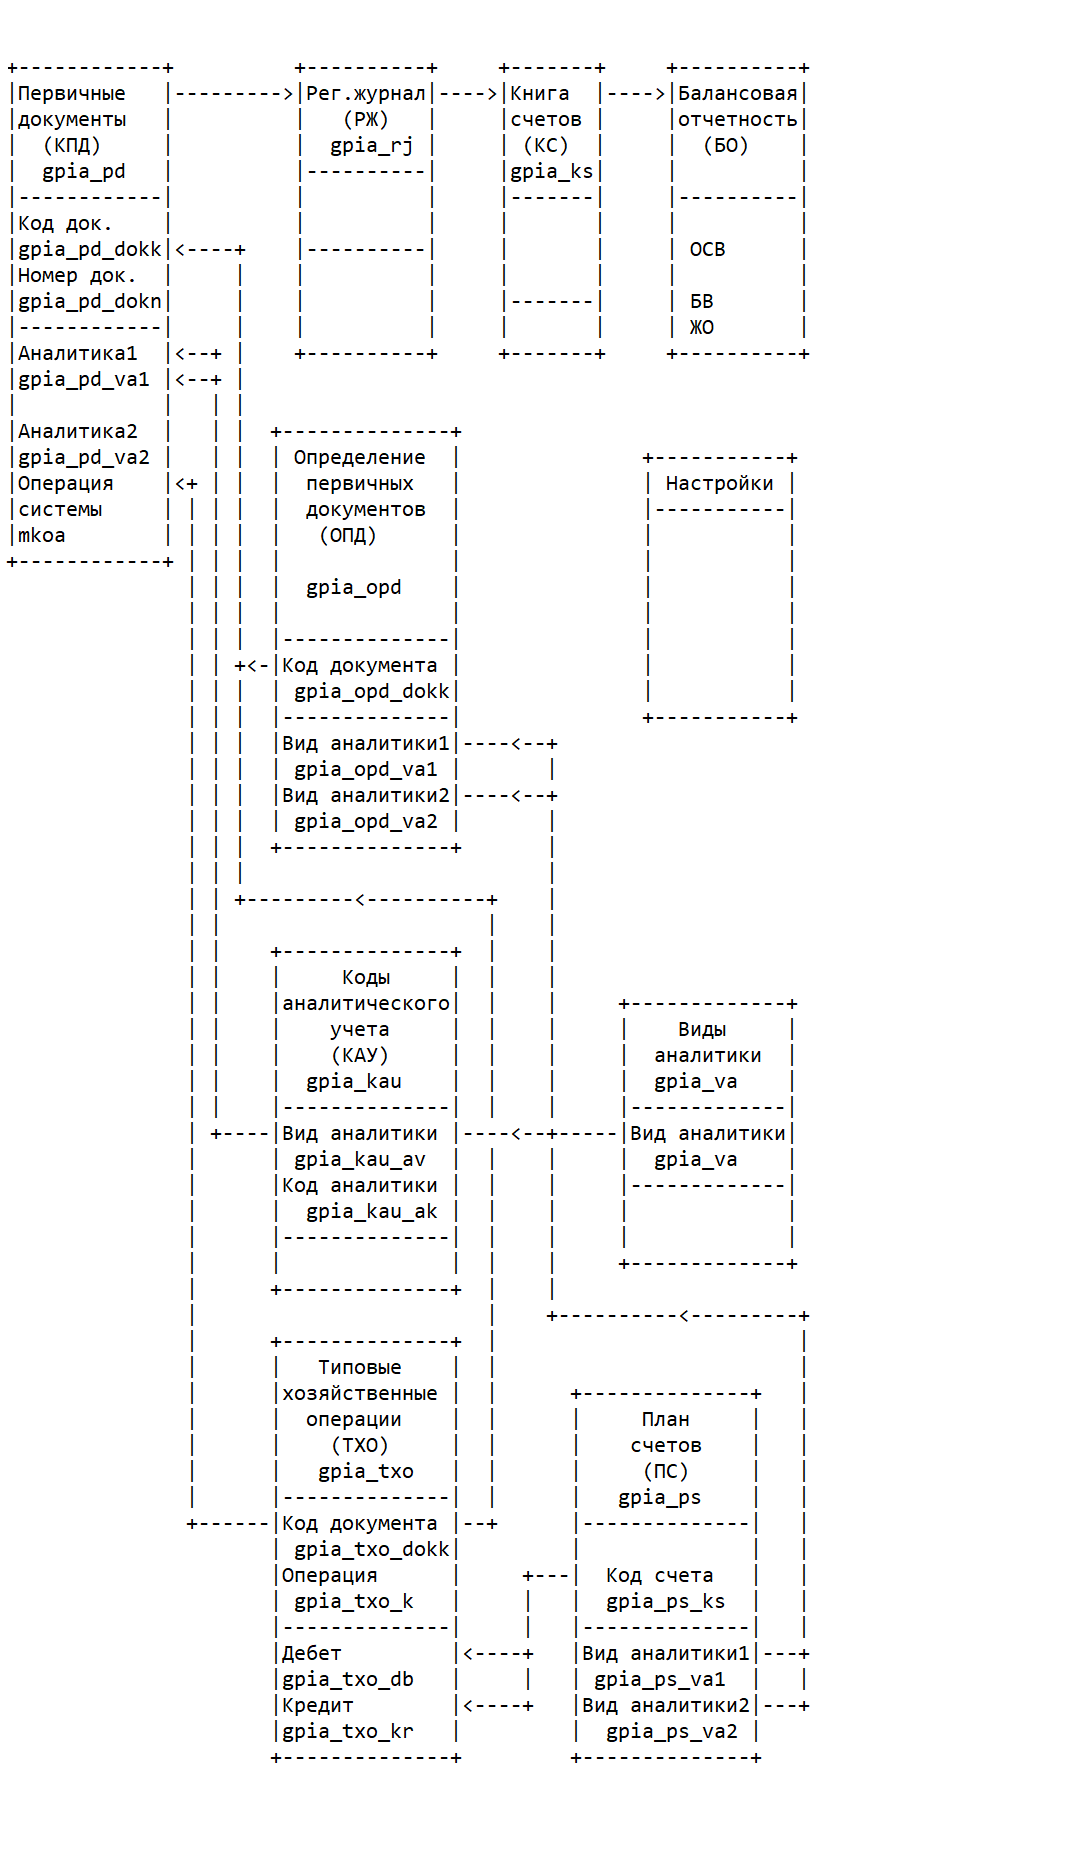
\includegraphics[height=19cm]
        {_assets/gpia_part2.png}
    \caption{Функциональная схема обработки данных}
\end{figure}

\subsection{Описание картотек}

Картотеки:

\begin{itemize}
    \item Первичные документы \gpiFIO\/a\_pd;
    \item[]\hspace{0pt}
    \item Регистрационный журнал (РЖ) \gpiFIO\/a\_rj;
    \item Книга счетов (КС) \gpiFIO\/a\_ks;
    \item[]\hspace{0pt}
    \item Определение первичных документов \gpiFIO\/a\_opd;
    \item Типовые хозяйственные операции (ТХО) \gpiFIO\/a\_txo;
    \item План счетов (ПС) \gpiFIO\/a\_ps;
    \item Коды аналитического учёта (КАУ) \gpiFIO\/a\_kau;
    \item Виды аналитики \gpiFIO\/a\_va;
    \item[]\hspace{0pt}
    \item Настройки системы \gpiFIO\/a\_nst;
\end{itemize}

\begin{table}[h!p]
    \centering
    \scriptsize
    \caption{Первичные документы \gpiFIO\/a\_pd}
    \begin{tabular}{|l|l|l|} 

\hline
\textbf{Реквизит}                   &\textbf{Обозначение}&\textbf{Тип и значность}  \\ \hline
поле связи               =0         &\gpiFIO\/a\_pd\_0        &c1                         \\ \hline
код документа    < --- opd          &\gpiFIO\/a\_pd\_dokk     &c3                         \\ \hline
номер документа                     &\gpiFIO\/a\_pd\_dokn     &n5                         \\ \hline
дата документа                      &\gpiFIO\/a\_pd\_dokd     &D                          \\ \hline
вид аналитики 1    *opd             &\gpiFIO\/a\_pd\_av1      &c3                         \\ \hline
тип аналитики 1      =д, к, x       &\gpiFIO\/a\_pd\_avt1     &c1                         \\ \hline
аналитика код 1   < --- kau         &\gpiFIO\/a\_pd\_ak1      &c10                        \\ \hline
вид аналитики2                      &\gpiFIO\/a\_pd\_av2      &c3                         \\ \hline
тип аналитики2                      &\gpiFIO\/a\_pd\_avt2     &c1                         \\ \hline
аналитика код2                      &\gpiFIO\/a\_pd\_ak2      &c10                        \\ \hline
вид аналитики3                      &\gpiFIO\/a\_pd\_av3      &c3                         \\ \hline
тип аналитики3                      &\gpiFIO\/a\_pd\_avt3     &c1                         \\ \hline
аналитика код3                      &\gpiFIO\/a\_pd\_ak3      &c10                        \\ \hline
операции                            &\gpiFIO\/a\_pd\_to       &c10                        \\ \hline
дебет счет *txo                     &\gpiFIO\/a\_pd\_db       &n2                         \\ \hline
дебет счет субсчет наименование *txo&\gpiFIO\/a\_pd\_dbn      &c10                        \\ \hline
кредит  *txo                        &\gpiFIO\/a\_pd\_kr       &n2                         \\ \hline
кредит название*txo                 &\gpiFIO\/a\_pd\_krn      &c10                        \\ \hline
сумма                               &\gpiFIO\/a\_pd\_rub      &n8                         \\ \hline
SAE                                 &\gpiFIO\/a\_pd\_sae      &c10                        \\ \hline

    \end{tabular}
\end{table}

\begin{table}[h!p]
    \centering
    \scriptsize
    \caption{Виды аналитики \gpiFIO\/a\_va}
    \begin{tabular}{|l|l|l|} 

                                                                               \hline
\textbf{Реквизит}       &\textbf{Обозначение}   &\textbf{Тип и значность}   \\ \hline
поле связи  	  =0    &\gpiFIO\/a\_va\_0            &c1                         \\ \hline
вид аналитики           &\gpiFIO\/a\_va\_k            &c3                         \\ \hline
название вида аналитики &\gpiFIO\/a\_va\_n            &c15                        \\ \hline

    \end{tabular}
\end{table}

\begin{table}[h!p]
    \centering
    \scriptsize
    \caption{Регистрационный журнал (РЖ) \gpiFIO\/a\_rj}
    \begin{tabular}{|l|l|l|} 

                                                                                   \hline
\textbf{Реквизит}           &\textbf{Обозначение}   &\textbf{Тип и значность}   \\ \hline
поле связи	=0              &\gpiFIO\/a\_rj\_0            &c1                         \\ \hline
дата операции               &\gpiFIO\/a\_rj\_data         &D                          \\ \hline
код оправдательного документа&\gpiFIO\/a\_rj\_dokk        &c3                         \\ \hline
номер документа             &\gpiFIO\/a\_rj\_dokn         &n5                         \\ \hline
дата документа              &\gpiFIO\/a\_rj\_dokd         &D                          \\ \hline
содержание операции         &\gpiFIO\/a\_rj\_to           &c10                        \\ \hline
дебет, счет                 &\gpiFIO\/a\_rj\_db           &n2                         \\ \hline
дебет, название             &\gpiFIO\/a\_rj\_dbn          &c10                        \\ \hline
кредит, счет                &\gpiFIO\/a\_rj\_kr           &n2                         \\ \hline
кредит название             &\gpiFIO\/a\_rj\_krn          &c10                        \\ \hline
SAE                         &\gpiFIO\/a\_rj\_sae          &c10                        \\ \hline
Сумма                       &\gpiFIO\/a\_rj\_rub          &n10                        \\ \hline

    \end{tabular}
\end{table}

\begin{table}[h!p]
    \centering
    \scriptsize
    \caption{Книга счетов(КС) \gpiFIO\/a\_ks}
    \begin{tabular}{|l|l|l|} 

                                                                                   \hline
\textbf{Реквизит}           &\textbf{Обозначение}   &\textbf{Тип и значность}   \\ \hline
поле связи  =0              &\gpiFIO\/a\_ks\_0      &c1                                 \\ \hline
дата операции               &\gpiFIO\/a\_ks\_data   &D                                  \\ \hline
код оправдательного документа&\gpiFIO\/a\_ks\_dokk  &c3                                 \\ \hline
номер документа             &\gpiFIO\/a\_ks\_dokn   &n5                                 \\ \hline
дата документа              &\gpiFIO\/a\_ks\_dokd   &D                                  \\ \hline
операции                    &\gpiFIO\/a\_ks\_to     &c10                                \\ \hline
счет                        &\gpiFIO\/a\_ks\_s      &n2                                 \\ \hline
счёт название               &\gpiFIO\/a\_ks\_sn     &c10                                \\ \hline
кор. счёт                   &\gpiFIO\/a\_ks\_ks     &n2                                 \\ \hline
кор. счет наименование      &\gpiFIO\/a\_ks\_ksn    &c10                                \\ \hline
сумма дб                    &\gpiFIO\/a\_ks\_db     &n10                                \\ \hline
сумма кр                    &\gpiFIO\/a\_ks\_kr     &n10                                \\ \hline
SAE                         &\gpiFIO\/a\_ks\_sae    &c10                                \\ \hline

    \end{tabular}
\end{table}

\begin{table}[h!p]
    \centering
    \scriptsize
    \caption{Определение первичных документов \gpiFIO\/a\_opd}
    \begin{tabular}{|l|l|l|} 

                                                                                   \hline
\textbf{Реквизит}           &\textbf{Обозначение}   &\textbf{Тип и значность}   \\ \hline
поле связи       =0         &\gpiFIO\/a\_opd\_0           &c1                         \\ \hline
код документа               &\gpiFIO\/a\_opd\_k           &c3                         \\ \hline
наименование документа      &\gpiFIO\/a\_opd\_n           &c10                        \\ \hline
вид аналитики 1  < ---  va  &\gpiFIO\/a\_opd\_av1         &c3                         \\ \hline
тип аналитики 1    =д, к, x &\gpiFIO\/a\_opd\_avt1        &c1                         \\ \hline
виды аналитики 2            &\gpiFIO\/a\_opd\_av2         &c3                         \\ \hline
тип аналитики 2             &\gpiFIO\/a\_opd\_avt2        &c1                         \\ \hline
вид аналитики 3             &\gpiFIO\/a\_opd\_av3         &c3                         \\ \hline
тип аналитики 2             &\gpiFIO\/a\_opd\_avt3        &c1                         \\ \hline

    \end{tabular}
\end{table}

\begin{table}[h!p]
    \centering
    \scriptsize
    \caption{Типовые хозяйственные операции(ТХО) \gpiFIO\/a\_txo}
    \begin{tabular}{|l|l|l|} 

                                                                                           \hline
\textbf{Реквизит}                   &\textbf{Обозначение}   &\textbf{Тип и значность}   \\ \hline
поле связи    =0                    &\gpiFIO\/a\_txo\_0           &c1                         \\ \hline
код документа        < ---  opd     &\gpiFIO\/a\_txo\_dokk        &c3                         \\ \hline
Операции                            &\gpiFIO\/a\_txo\_k           &c10                        \\ \hline
дебет, счёт            < ---  ps\_1 &\gpiFIO\/a\_txo\_db          &n2                         \\ \hline
дебет, название       * ps\_1       &\gpiFIO\/a\_txo\_dbn         &c10                        \\ \hline
кредит                   < --- ps\_2&\gpiFIO\/a\_txo\_kr          &n2                         \\ \hline
кредит, название    * ps\_2         &\gpiFIO\/a\_txo\_krn         &c10                        \\ \hline
SAE                                 &\gpiFIO\/a\_txo\_sae         &c10                        \\ \hline

    \end{tabular}
\end{table}

\begin{table}[h!p]
    \centering
    \scriptsize
    \caption{План счетов(ПС) \gpiFIO\/a\_ps}
    \begin{tabular}{|l|l|l|} 

                                                                                           \hline
\textbf{Реквизит}                   &\textbf{Обозначение}   &\textbf{Тип и значность}   \\ \hline
поле связи        =0                &\gpiFIO\/a\_ps\_0            &c1                         \\ \hline
счет                                &\gpiFIO\/a\_ps\_s            &n2                         \\ \hline
название счета                      &\gpiFIO\/a\_ps\_n            &c10                        \\ \hline
тип счета          = а, п, x        &\gpiFIO\/a\_ps\_typ          &c1                         \\ \hline
вид аналитики 1 из VA               &\gpiFIO\/a\_ps\_av1          &c3                         \\ \hline
вид аналитики 2 из VA               &\gpiFIO\/a\_ps\_av2          &c3                         \\ \hline

    \end{tabular}
\end{table}

\begin{table}[h!p]
    \centering
    \scriptsize
    \caption{Коды аналитического учёта(КАУ) \gpiFIO\/a\_kau}
    \begin{tabular}{|l|l|l|} 

                                                                               \hline
\textbf{Реквизит}       &\textbf{Обозначение}   &\textbf{Тип и значность}   \\ \hline
поле связи          =0  &\gpiFIO\/a\_kau\_0           &c1                         \\ \hline
вид аналитики           &\gpiFIO\/a\_kau\_k           &c5                         \\ \hline
вид аналитики           &\gpiFIO\/a\_kau\_n           &c15                        \\ \hline

    \end{tabular}
\end{table}

\begin{table}[h!p]
    \centering
    \scriptsize
    \caption{Настройки системы \gpiFIO\/a\_nst}
    \begin{tabular}{|l|l|l|} 

                                                                               \hline
\textbf{Реквизит}       &\textbf{Обозначение}   &\textbf{Тип и значность}   \\ \hline
поле связи          =0  &\gpiFIO\/a\_nst\_0           &c1                         \\ \hline
дата текущая            &\gpiFIO\/a\_nst\_datat       &D                          \\ \hline
интервал с              &\gpiFIO\/a\_nst\_datas       &D                          \\ \hline
интервал до             &\gpiFIO\/a\_nst\_datado      &D                          \\ \hline
cчёт                    &\gpiFIO\/a\_nst\_s           &n2                         \\ \hline
название счёта          &\gpiFIO\/a\_nst\_sn          &c10                        \\ \hline
название фирмы          &\gpiFIO\/a\_nst\_firma       &c10                        \\ \hline

    \end{tabular}
\end{table}

\subsection{Описание работ}

\begin{table}[h!p]
    \centering
    \scriptsize
    \caption{Описание работ}
    \begin{tabular}{|p{8cm}|p{9cm}|} 

% = = = = = = = = = =

\hline

% = = = = = = = = = =

\textbf{Группа работ}
&
\textbf{Работы}
\\ \hline

% = = = = = = = = = =

Формирование и разноска первичных документов \par
\hspace{0pt} \par
\textbf{\gpiFIO\/a\_Документы}
&
- \gpiFIO\/a\_Ввод текущей даты \par
- \gpiFIO\/a\_Ввод и разноска первичных документов
\\ \hline

% = = = = = = = = = =

Работа с регистрационным журналом \par
\hspace{0pt} \par
\textbf{\gpiFIO\/a\_РЖ}
&
- \gpiFIO\/a\_Просмотр РЖ \par
- \gpiFIO\/a\_Просмотр РЖ (запрос) \par
- \gpiFIO\/a\_Формирование книги счетов из рег. журнала \par
- \gpiFIO\/a\_Просмотр КС \par
- \gpiFIO\/a\_Просмотр КС (запрос) \par
- \gpiFIO\/a\_Печать книги счетов
\\ \hline

% = = = = = = = = = =

Формирование балансовой отчетности \par
\hspace{0pt} \par
\textbf{\gpiFIO\/a\_БО}
&
- \gpiFIO\/a\_Опеделение форм \par
- \gpiFIO\/a\_Оборотно-сальдовая ведомость за период... по счету... \par
- \gpiFIO\/a\_Балансовая ведомость по счету за период... по счету... \par
- \gpiFIO\/a\_Журнал-ордер за период... по счету...
\\ \hline

% = = = = = = = = = =

Сопровождение картотек-справочников \par
\hspace{0pt} \par
\textbf{\gpiFIO\/a\_Картотеки}
&
- \gpiFIO\/a\_Определение первичных документов \par
- \gpiFIO\/a\_Типовые хозяйственные операции(ТХО) \par
- \gpiFIO\/a\_План счетов(ПС) \par
- \gpiFIO\/a\_Виды аналитики \par
- \gpiFIO\/a\_Коды аналитического учёта(КАУ) \par
- \gpiFIO\/a\_Настройка АРМа
\\ \hline

% = = = = = = = = = =

Ведение архивов \par
\hspace{0pt} \par
\textbf{\gpiFIO\/a\_Архивы}
&
- \gpiFIO\/a\_Копирование системы!!! \par
- \gpiFIO\/a\_Восстановление системы!!!
\\ \hline

% = = = = = = = = = =

Выход из системы \par
\hspace{0pt} \par
\textbf{\gpiFIO\/a\_Выход}
&
- \gpiFIO\/a\_Выход из системы
\\ \hline

% = = = = = = = = = =

    \end{tabular}
\end{table}

\newpage
